\chapter{Geometry}

\section{Q1}

  \begin{figure}[H]
    \centering
    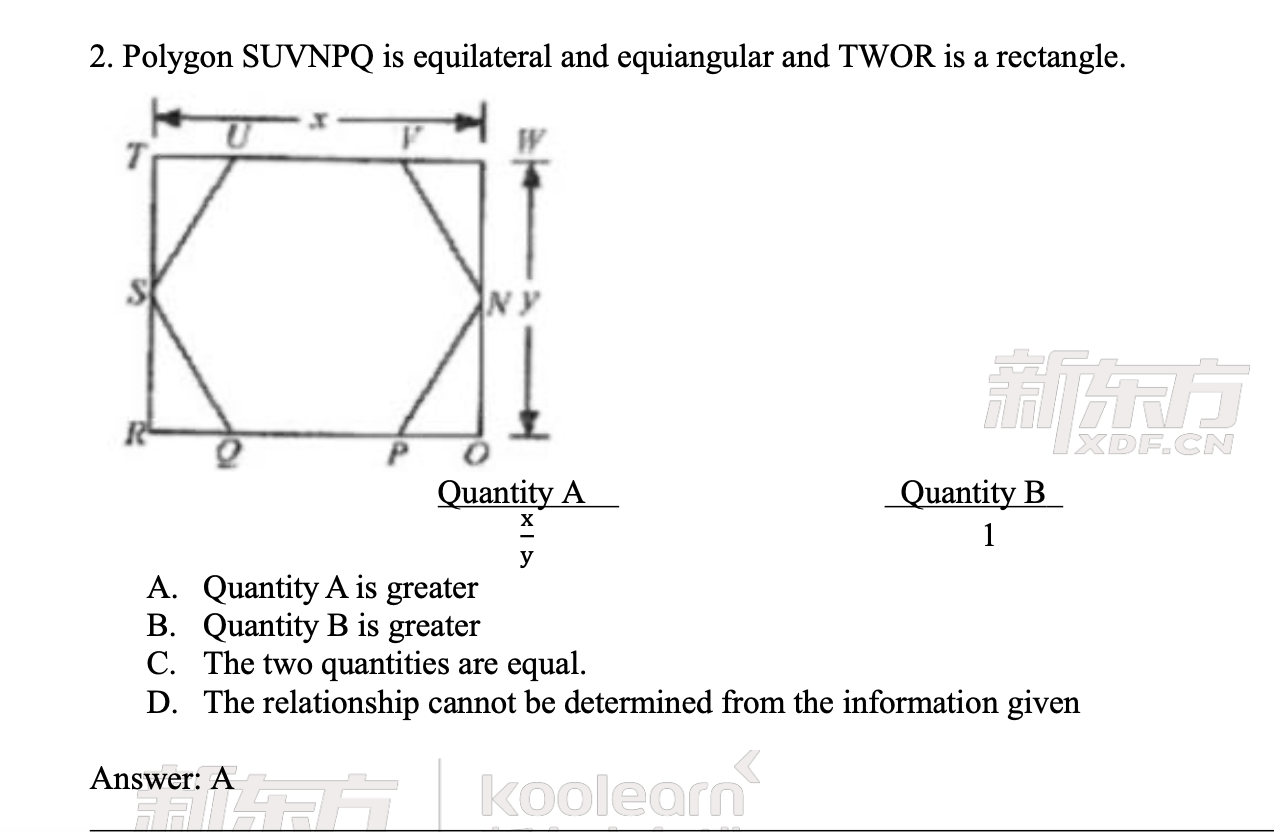
\includegraphics[width=0.7\columnwidth]{images/areas/geometry/q1}
  \end{figure}

\section{Q2}

  If $ x > 0 $, and two sides of a certain triangle have lengths $ 2 x + 1 $
  and $ 3 x + 4 $ respectively, which of the following could be the length of
  the third side of the triangle? (多选题)

  \begin{enumerate}
    \item $ 4x + 5 $
    \item $ x + 2 $
    \item $ 6x + 1 $
    \item $ 5x + 6 $
    \item $ 2x + 17 $
  \end{enumerate}

  \subsection{解析}

    本题考查三角形两边之和大于第三边, 注意\textbf{could be}

    \textbf{答案}: A, C, E

\section{Q3}

  \begin{figure}[H]
    \centering
    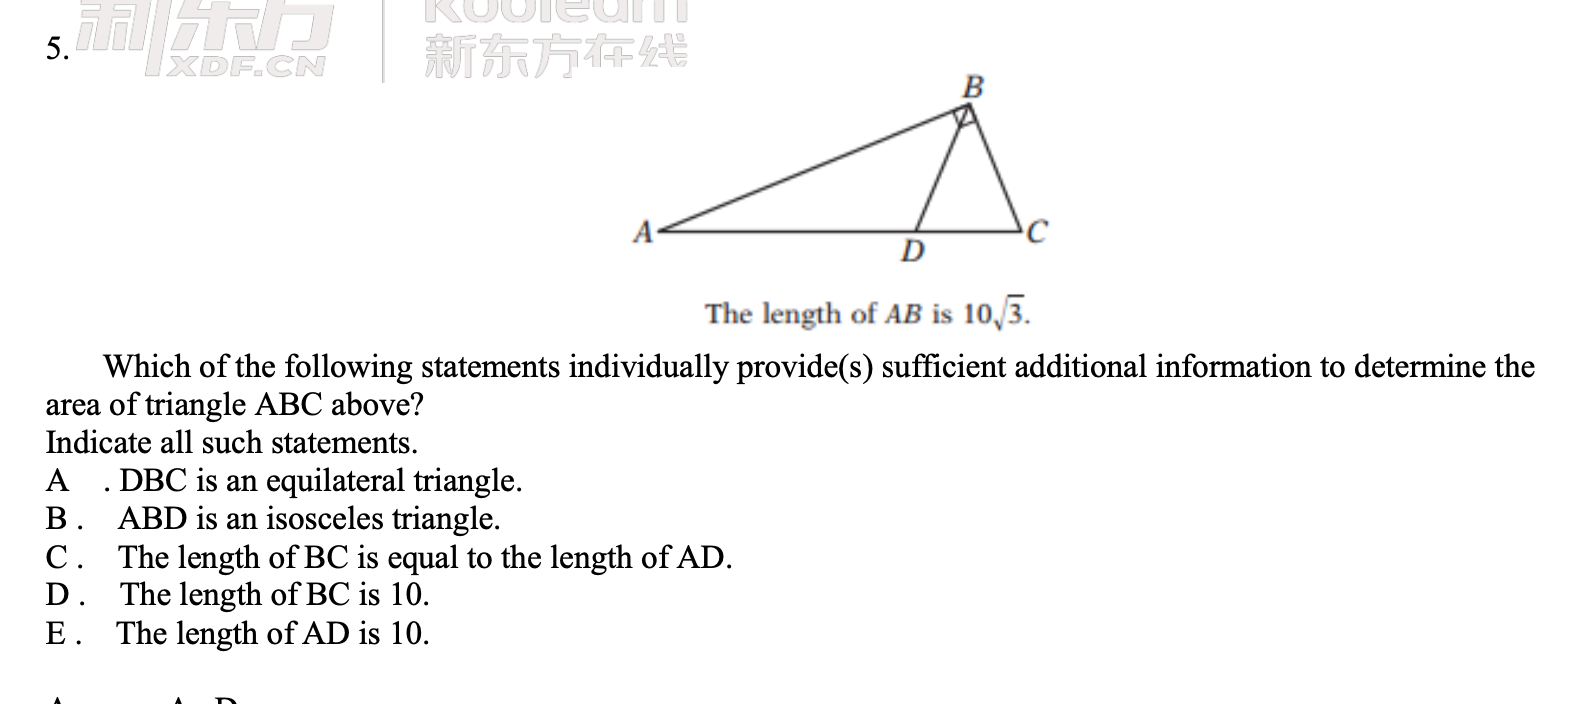
\includegraphics[width=0.7\columnwidth]{images/areas/geometry/q3}
  \end{figure}

  \textbf{多选题}

  \subsection{解析}

    主要目标位找到$ BC $

    \begin{itemize}
      \item \textbf{A}: 等边三角形, 30度所对直角边为斜边的一半,
      $ BC = DC = \frac{AC}{2} $, 解方程可得 $ BC $
    \end{itemize}

    \textbf{答案 A, D}

\section{Q4}

  \begin{figure}[H]
    \centering
    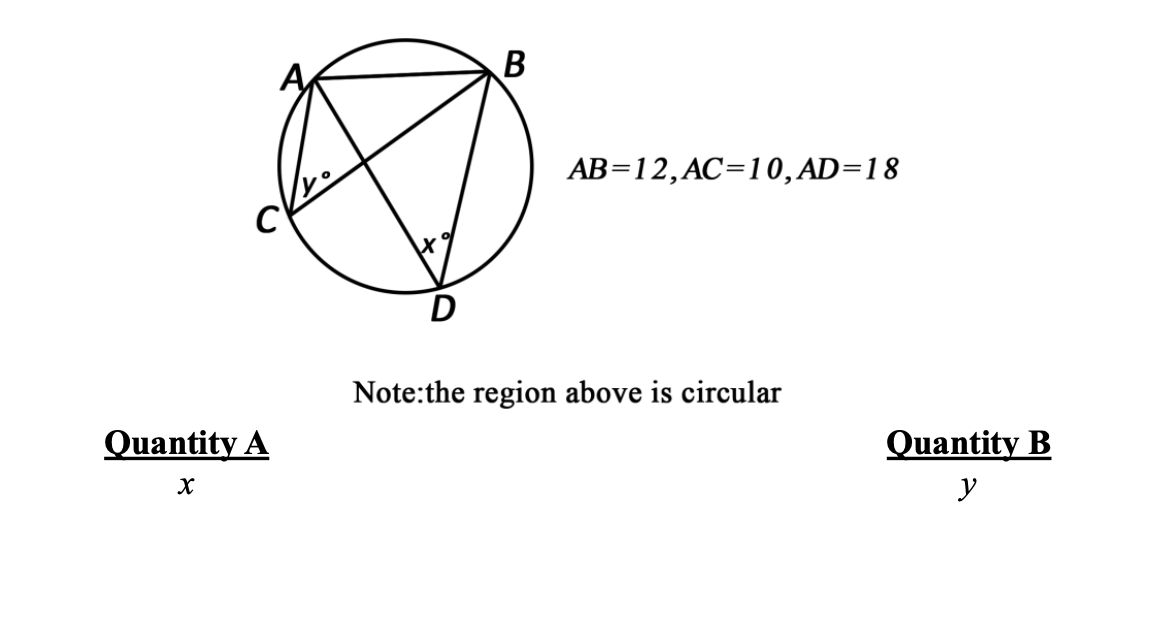
\includegraphics[width=0.7\columnwidth]{images/areas/geometry/q4}
  \end{figure}

  \subsection{解析}

    \textbf{C}, 同圆弧的圆周角相等

\section{Q5}

  If the length of each side of an equilateral triangle were increased by
  50 percent, what would be the percent increase in the area?

  \subsection{解析}

    等边三角形的底和高都涉及到边, 所以面积和 $ x^{2} $成比例

    \begin{align*}
      1.5 \times 1.5 - 1 &= 2.25 - 1 \\
      &= 1.25
    \end{align*}

    \textbf{本题注意审题, 最后一定要剪1}

\section{Q6}

  \begin{figure}[H]
    \centering
    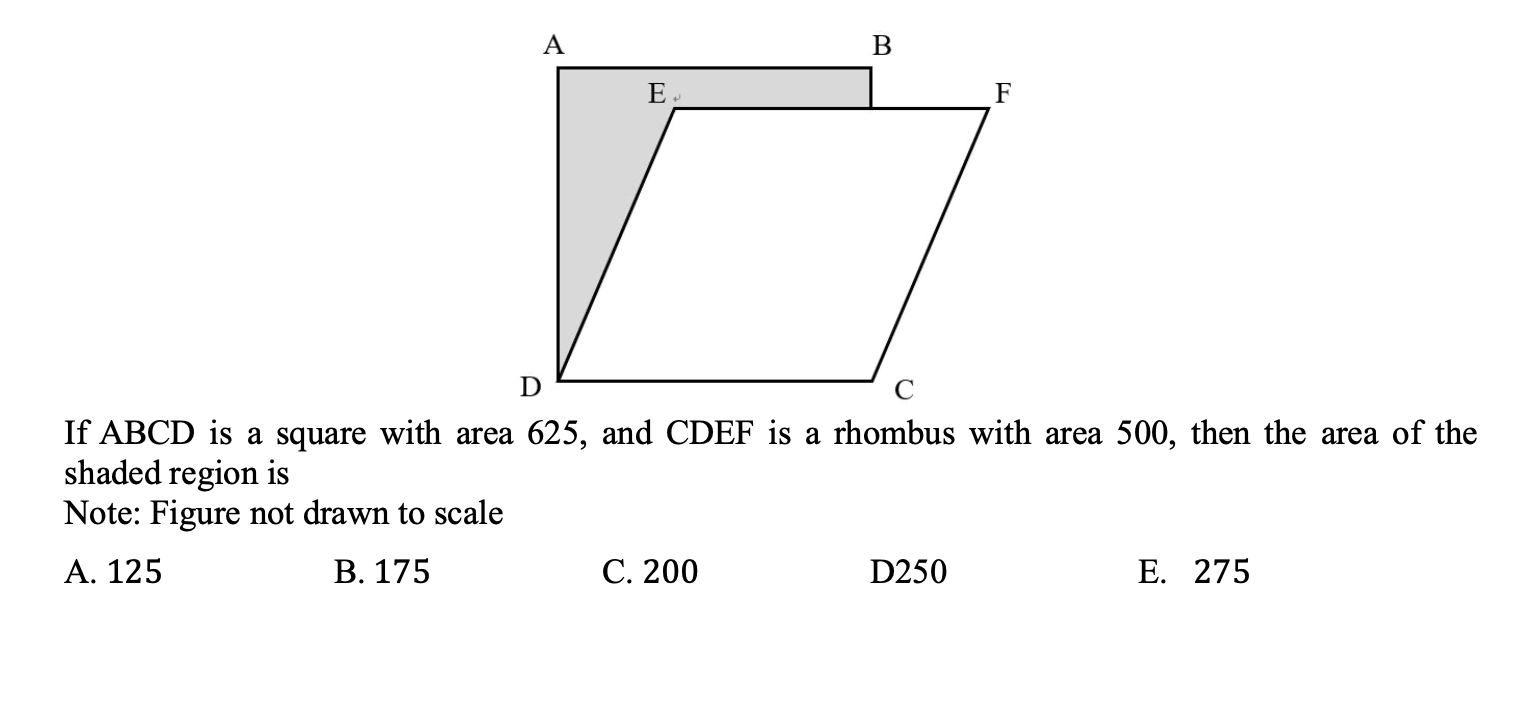
\includegraphics[width=0.7\columnwidth]{images/areas/geometry/q6}
  \end{figure}

  \subsection{解析}

    \begin{align*}
      A &=
      \left( 625 - 500 \right)
      + \left( \sqrt{625}^{2}
        - \left( \frac{500}{\sqrt{625}} \right)^{2}
        \right)
      \times \left( \frac{500}{\sqrt{625}} \right)
      \times 0.5 \\
      &= 125 + 250 \\
      &= 275
    \end{align*}

    \textbf{本文主要考察菱形的四边相等}

\section{Q7}

  \begin{figure}[H]
    \centering
    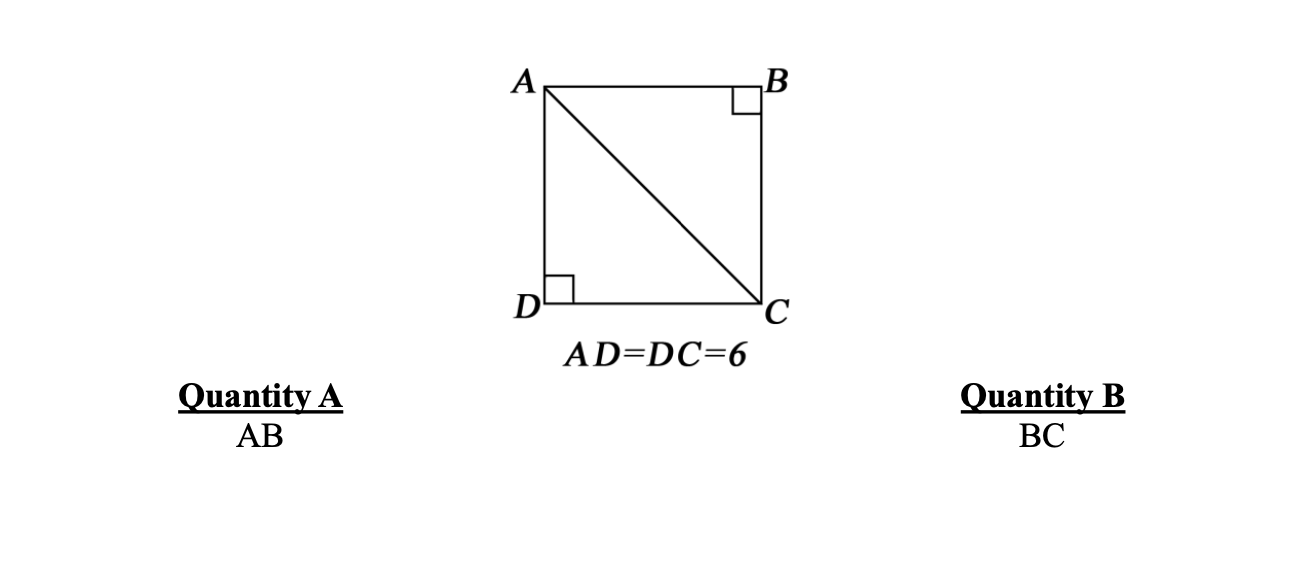
\includegraphics[width=0.7\columnwidth]{images/areas/geometry/q7}
  \end{figure}

  \subsection{解析}

    从给出的信息只能得到 $ DAC, DCA $的角度, $ DAB, BCD $的角度不知道, 所以无法
    得出结论

    \textbf{只能从文中所给信息推倒}

\section{Q8}

  \begin{figure}[H]
    \centering
    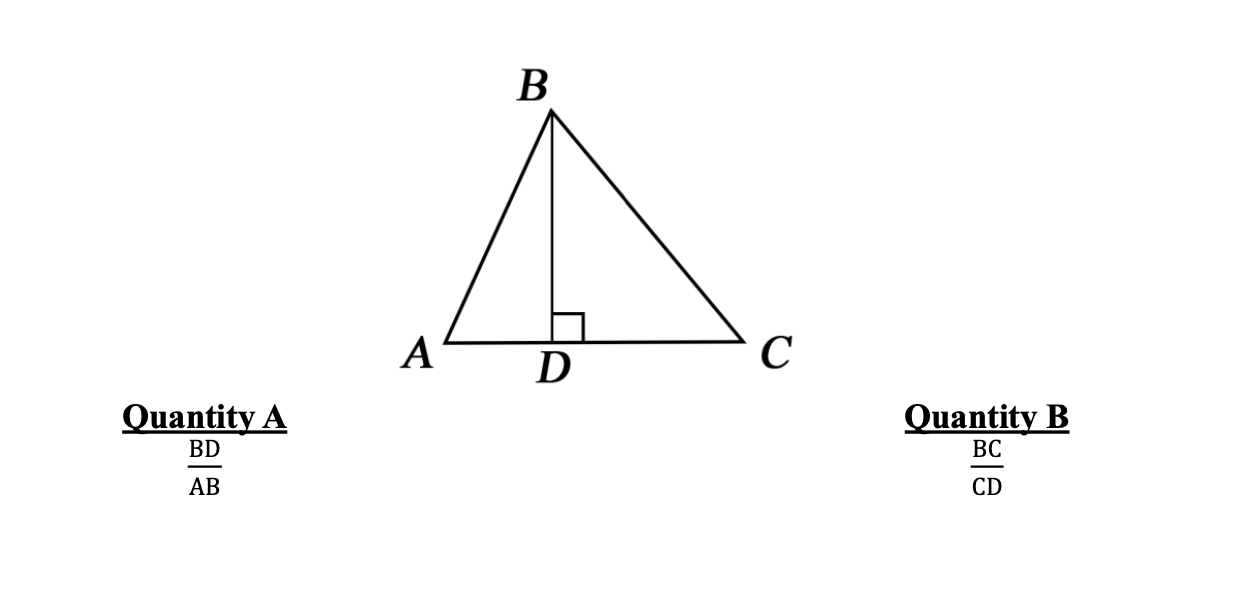
\includegraphics[width=0.7\columnwidth]{images/areas/geometry/q8}
  \end{figure}

  \subsection{解析}

    BD比AB短, BC比CD长(勾股定理), \textbf{答案 B}

\section{Q9}

  If we use some rectangular solids with edges 7cm, 3cm, and 2cm to form a
  solid cube, what is the least possible length of the edge of the cube?

  \subsection{解析}

    找LCM (为什么不知道), $ 42 $
